%% Manuscript for the International Journal of Systems Science: Operations & Logistics.
%% Every number comes from generated macros or generated tables
%% (code/ijss_tables.py, code/nhsjs_tables.py, code/itor_tables.py, code/analyse_v7.py ... analyse_v12.py).
\documentclass[11pt,a4paper]{article}
\usepackage[margin=2.5cm]{geometry}
\usepackage{mathptmx}
\usepackage{amsmath,amssymb,amsthm,booktabs,array,graphicx,microtype}
\usepackage{setspace}
\usepackage{caption}
\captionsetup{labelfont=bf,labelsep=period,font=small}
\usepackage[round,authoryear]{natbib}
\usepackage{url}
\usepackage[hidelinks]{hyperref}
\newtheorem{theorem}{Theorem}
\newtheorem{lemma}{Lemma}
\newtheorem{corollary}{Corollary}
\newtheorem{proposition}{Proposition}
\theoremstyle{remark}
\newtheorem{remark}{Remark}
\newif\ifanonymous
\anonymousfalse
\newcommand{\refsfile}{ijss_refs}
% the review copy (no identifying information) is built by code/build_ijss.py, which defines \anonbuild
\ifdefined\anonbuild \anonymoustrue \renewcommand{\refsfile}{ijss_refs_anon}\fi

\newcommand{\ProcConsRange}{8.3--21.4}
\newcommand{\ConservativeSelected}{25}
\newcommand{\ConservativeRetained}{25}
\newcommand{\CappedSelected}{42}
\newcommand{\CappedRetained}{40}
\newcommand{\OriginalRetained}{30}
\newcommand{\OriginalProbability}{78.9}
\newcommand{\ConservativeProbability}{78.6}
\newcommand{\CappedProbability}{86.6}
\newcommand{\ClockFound}{49}
\newcommand{\CappedGainInterval}{7.7 [3.5, 12.5]}
\newcommand{\CappedDistanceCost}{2.5}
\newcommand{\CappedFleetCost}{0.43}
\newcommand{\OriginalSelected}{32}
\newcommand{\FailureCount}{21}
\newcommand{\CertifiedFailures}{17}
\newcommand{\SweepLowIndep}{-3.1}
\newcommand{\SweepHighIndep}{30.5}
\newcommand{\CappedLargeRange}{97.5--97.6}
\newcommand{\CappedLargeSelected}{18/18}
\newcommand{\CappedLargeRetained}{16/18}
\newcommand{\OriginalSelectedMean}{97.3}
\newcommand{\OriginalFallbackMean}{50.9}
\newcommand{\CappedSelectedMean}{97.4}
\newcommand{\CappedFallbackMean}{45.2}
\newcommand{\CappedFallbackCount}{11}
\newcommand{\BudgetDiagCases}{8}
\newcommand{\BudgetDiagSearchLimits}{4}
\newcommand{\BudgetDiagUnresolved}{4}
\newcommand{\CappedFleetLarge}{1.88}
\newcommand{\ConfInstances}{53}
\newcommand{\ConfCommon}{50}
\newcommand{\ConfHOneMean}{15.7}
\newcommand{\ConfHOneLo}{7.5}
\newcommand{\ConfHOneHi}{23.6}
\newcommand{\ConfHTwoMean}{11.7}
\newcommand{\ConfHTwoLo}{5.9}
\newcommand{\ConfHTwoHi}{17.9}
\newcommand{\ConfHThreeK}{46}
\newcommand{\ConfHThreeP}{32}
\newcommand{\ConfHThreeKonly}{14}
\newcommand{\ConfHThreePonly}{0}
\newcommand{\ConfHThreeExact}{0.00012}
\newcommand{\ConfHFourMean}{28.3}
\newcommand{\ConfHFourLo}{19.6}
\newcommand{\ConfHFourHi}{36.4}
\newcommand{\ConfPooledP}{79.4}
\newcommand{\ConfPooledSC}{82.4}
\newcommand{\ConfPooledK}{91.0}
\newcommand{\ConfRetainedP}{31/32}
\newcommand{\ConfRetainedK}{45/46}
\newcommand{\ConfNoPlanConservative}{3}
\newcommand{\ConfNoPlanClock}{4}
\newcommand{\ConfAdmMeanP}{97.4}
\newcommand{\ConfFbMeanP}{51.9}
\newcommand{\ConfFbCountP}{21}
\newcommand{\ConfAdmMeanK}{97.5}
\newcommand{\ConfFbMeanK}{48.7}
\newcommand{\ConfFbCountK}{7}
\newcommand{\PostHocP}{85.0}
\newcommand{\PostHocK}{93.0}
\newcommand{\PostHocChangedP}{18}
\newcommand{\PostHocChangedK}{6}
\newcommand{\HTwoFromKonly}{11.6}
\newcommand{\WtEqualDiffMean}{$-$8.8}
\newcommand{\WtEqualDiffLo}{$-$14.3}
\newcommand{\WtEqualDiffHi}{$-$3.5}
\newcommand{\WtEqualPCMean}{6.3}
\newcommand{\WtEqualPCLo}{$-$1.1}
\newcommand{\WtEqualPCHi}{13.7}
\newcommand{\WtEqualAdmitted}{23}
\newcommand{\WtBaseAdmitted}{31}
\newcommand{\WtDistanceHeavyPCMean}{12.7}
\newcommand{\WtDistanceHeavyPCLo}{5.3}
\newcommand{\WtDistanceHeavyPCHi}{19.7}
\newcommand{\SolomonN}{8}
\newcommand{\SolomonPlans}{5}
\newcommand{\SolomonAdmitted}{3}
\newcommand{\SolomonNoPlan}{3}

\newcommand{\CtwoGOneMean}{28.0}
\newcommand{\CtwoGOneLo}{23.0}
\newcommand{\CtwoGOneHi}{32.8}
\newcommand{\CtwoGTwoMean}{0.4}
\newcommand{\CtwoGTwoLo}{$-$0.7}
\newcommand{\CtwoGTwoHi}{2.1}
\newcommand{\CtwoGThreeMean}{3.8}
\newcommand{\CtwoGThreeLo}{1.6}
\newcommand{\CtwoGThreeHi}{6.2}
\newcommand{\CtwoGFourMean}{$-$0.2}
\newcommand{\CtwoGFourLo}{$-$4.0}
\newcommand{\CtwoGFourHi}{3.7}
\newcommand{\CtwoCommon}{49}
\newcommand{\CtwoPooledHGSCons}{58.4}
\newcommand{\CtwoPooledHGSK}{91.6}
\newcommand{\CtwoPooledORTK}{91.4}
\newcommand{\CtwoPooledORTKc}{91.7}
\newcommand{\CtwoORTKAdmitted}{45}
\newcommand{\CtwoORTKFallbacks}{8}
\newcommand{\CtwoFallbacksChanged}{4}
\newcommand{\CtwoHGSKAdmittedLarge}{18}
\newcommand{\CtwoHGSPAdmittedLarge}{3}
\newcommand{\CtwoLarge}{18}
\newcommand{\DevHGSGOneMean}{27.0}
\newcommand{\DevHGSGOneLo}{23.0}
\newcommand{\DevHGSGOneHi}{30.8}
\newcommand{\DevHGSPooledK}{94.2}

\newcommand{\RobInstances}{45}
\newcommand{\RobNoPlanBoxFour}{8}
\newcommand{\RobNoPlanBoxSix}{16}
\newcommand{\RobBoxFourP}{75.0}
\newcommand{\RobBoxSixP}{63.3}
\newcommand{\RobCapGThreeFourP}{89.4}
\newcommand{\RobCapBoxFourP}{91.4}
\newcommand{\RobCapGThreeSixP}{97.8}
\newcommand{\RobCapBoxSixP}{98.4}
\newcommand{\RobScreenedP}{87.4}
\newcommand{\RobScreenedCapP}{97.2}
\newcommand{\RobScreenedCapAdm}{44}
\newcommand{\RobScreenedAdm}{29}
\newcommand{\RobOrtCappedP}{84.6}
\newcommand{\RobHgsCappedP}{93.6}
\newcommand{\RobOrtNominalD}{1.7}
\newcommand{\RobReliefGain}{16.4}
\newcommand{\RobCapGThreeFourMinusOrt}{4.8}
\newcommand{\RobCapGThreeFourMinusOrtLo}{$-$1.4}
\newcommand{\RobCapGThreeFourMinusOrtHi}{11.6}
\newcommand{\RobCapGThreeFourMinusOrtFleet}{0.42}
\newcommand{\RobCapGThreeSixMinusHgs}{4.2}
\newcommand{\RobCapGThreeSixMinusHgsLo}{1.3}
\newcommand{\RobCapGThreeSixMinusHgsHi}{7.7}
\newcommand{\RobCapGThreeSixMinusHgsFleet}{0.67}
\newcommand{\RobScreenedCapMinusHgs}{3.6}
\newcommand{\RobScreenedCapMinusHgsLo}{0.6}
\newcommand{\RobScreenedCapMinusHgsHi}{7.1}
\newcommand{\RobScreenedCapMinusHgsFleet}{0.53}
\newcommand{\RobBenchEqualTwenty}{20}
\newcommand{\RobBenchCountTwenty}{20}
\newcommand{\RobBenchGapFifty}{0.04}
\newcommand{\RobBenchGapHundred}{0.9}
\newcommand{\RobItersSmall}{6000}
\newcommand{\RobItersHundred}{3000}

\newcommand{\FwAdmittedOrig}{318}
\newcommand{\FwAdmittedTotal}{306}
\newcommand{\FwMissOrig}{11}
\newcommand{\FwMissFw}{1}
\newcommand{\FwLostMax}{2}
\newcommand{\FwPooledChangeMin}{$-$1.8}
\newcommand{\FwPooledChangeMax}{0.2}
\newcommand{\FwAdmMeanMin}{97.7}
\newcommand{\FwAdmMeanMax}{98.3}
\newcommand{\AdmMeanMin}{97.3}
\newcommand{\AdmMeanMax}{98.0}
\newcommand{\TimeScreenTwenty}{3}
\newcommand{\TimeScreenTwoHundred}{24}
\newcommand{\TimeHgsTwenty}{2.2}
\newcommand{\TimeHgsTwoHundred}{9.3}
\newcommand{\BetaOrtMid}{191}
\newcommand{\BetaOrtN}{225}
\newcommand{\BetaOrtEdge}{4}
\newcommand{\BetaHgsEdge}{11}
\newcommand{\BetaHgsN}{93}
\newcommand{\MisMinOrig}{11.5}
\newcommand{\MisMinOrt}{21.9}
\newcommand{\MisMinHgs}{23.3}
\newcommand{\MisCappedDrop}{6.9}
\newcommand{\MisConsDrop}{21.2}
\newcommand{\MisKOrt}{159}
\newcommand{\MisKHgs}{106}
\newcommand{\MisKRob}{45}

\newcommand{\FbGainMin}{3.0}
\newcommand{\FbGainMax}{15.6}
\newcommand{\FbCappedPooledMin}{95.1}
\newcommand{\FbCappedPooledMax}{97.2}
\newcommand{\PbFOne}{7.3}
\newcommand{\PbFOneLo}{2.3}
\newcommand{\PbFOneHi}{13.2}
\newcommand{\PbFTwo}{4.2}
\newcommand{\PbFTwoLo}{1.2}
\newcommand{\PbFTwoHi}{8.0}
\newcommand{\PbFThree}{94.4}
\newcommand{\PbFThreeLo}{90.1}
\newcommand{\PbFThreeHi}{97.1}
\newcommand{\PbFFour}{94.9}
\newcommand{\PbFFourLo}{91.0}
\newcommand{\PbFFourHi}{97.1}
\newcommand{\PbInstances}{53}
\newcommand{\PbOrtFallbacks}{9}
\newcommand{\PbHgsFallbacks}{8}
\newcommand{\PbOrtPooled}{87.1}
\newcommand{\PbHgsPooled}{90.7}
\newcommand{\PbNoAnchor}{1}
\newcommand{\PbExOrt}{96.3}
\newcommand{\PbExHgs}{96.7}
\newcommand{\PaROne}{6.7}
\newcommand{\PaROneLo}{3.0}
\newcommand{\PaROneHi}{11.1}
\newcommand{\PaRTwo}{6.7}
\newcommand{\PaRTwoLo}{2.2}
\newcommand{\PaRTwoHi}{12.2}
\newcommand{\PaRThree}{0.42}
\newcommand{\PaRFour}{$-$1.3}
\newcommand{\PaRFourAbs}{1.3}
\newcommand{\PaBoxMinusScr}{1.2}
\newcommand{\PaInstances}{90}
\newcommand{\PaScreenedP}{97.2}
\newcommand{\PaOrtP}{90.5}
\newcommand{\PaHgsP}{90.6}
\newcommand{\PaBoxP}{98.4}
\newcommand{\PaAdmitted}{86}
\newcommand{\FmHgs}{$-$1.9}
\newcommand{\FmHgsLo}{$-$5.1}
\newcommand{\FmHgsHi}{1.5}
\newcommand{\FmConfHgs}{3.2}
\newcommand{\FmConfHgsLo}{$-$1.1}
\newcommand{\FmConfHgsHi}{8.1}
\newcommand{\FmConfOrt}{$-$0.7}
\newcommand{\FmConfOrtLo}{$-$3.9}
\newcommand{\FmConfOrtHi}{2.7}
\newcommand{\BrOrigAdv}{17.5}
\newcommand{\BrEqAdv}{8.1}
\newcommand{\BrEqAdvLo}{1.1}
\newcommand{\BrEqAdvHi}{15.1}
\newcommand{\BrDurDiff}{$-$8.9}
\newcommand{\BrFleetDiff}{$-$5.6}
\newcommand{\BrEqDiff}{$-$8.5}
\newcommand{\GhAdmitted}{17}
\newcommand{\GhAttempted}{18}
\newcommand{\GhDiff}{15.1}
\newcommand{\GhDiffLo}{11.0}
\newcommand{\GhDiffHi}{19.1}
\newcommand{\GhCapped}{87.2}
\newcommand{\GhCons}{73.6}

\newcommand{\PaRThreeLo}{0.20}
\newcommand{\PaRThreeHi}{0.67}
\newcommand{\PaRFourLo}{$-$1.7}
\newcommand{\PaRFourHi}{$-$0.9}
\newcommand{\ItorCostDistRange}{2.0--4.9}

\newcommand{\PadInstances}{53}
\newcommand{\PadCapPooled}{86.6}
\newcommand{\PadBestLevel}{30}
\newcommand{\PadBestPooled}{66.7}
\newcommand{\PadBestDiff}{$-$19.9}
\newcommand{\PadBestDiffLo}{$-$28.8}
\newcommand{\PadBestDiffHi}{$-$11.7}
\newcommand{\PadZeroPooled}{21.9}
\newcommand{\PadZeroPlans}{53}
\newcommand{\PadZeroNoPlan}{0}
\newcommand{\PadZeroOnPlans}{21.9}
\newcommand{\PadZeroCapOnPlans}{86.6}
\newcommand{\PadZeroDiff}{$-$64.7}
\newcommand{\PadZeroDiffLo}{$-$70.2}
\newcommand{\PadZeroDiffHi}{$-$58.8}
\newcommand{\PadZeroDist}{$-$7.1}
\newcommand{\PadZeroDistAbs}{7.1}
\newcommand{\PadZeroFleet}{$-$0.89}
\newcommand{\PadTenPooled}{43.7}
\newcommand{\PadTenPlans}{51}
\newcommand{\PadTenNoPlan}{2}
\newcommand{\PadTenOnPlans}{45.4}
\newcommand{\PadTenCapOnPlans}{88.4}
\newcommand{\PadTenDiff}{$-$42.9}
\newcommand{\PadTenDiffLo}{$-$48.0}
\newcommand{\PadTenDiffHi}{$-$37.4}
\newcommand{\PadTenDist}{$-$6.2}
\newcommand{\PadTenDistAbs}{6.2}
\newcommand{\PadTenFleet}{$-$0.59}
\newcommand{\PadTwentyPooled}{56.8}
\newcommand{\PadTwentyPlans}{46}
\newcommand{\PadTwentyNoPlan}{7}
\newcommand{\PadTwentyOnPlans}{65.4}
\newcommand{\PadTwentyCapOnPlans}{89.4}
\newcommand{\PadTwentyDiff}{$-$23.9}
\newcommand{\PadTwentyDiffLo}{$-$29.2}
\newcommand{\PadTwentyDiffHi}{$-$18.2}
\newcommand{\PadTwentyDist}{$-$4.8}
\newcommand{\PadTwentyDistAbs}{4.8}
\newcommand{\PadTwentyFleet}{$-$0.22}
\newcommand{\PadThirtyPooled}{66.7}
\newcommand{\PadThirtyPlans}{43}
\newcommand{\PadThirtyNoPlan}{10}
\newcommand{\PadThirtyOnPlans}{82.2}
\newcommand{\PadThirtyCapOnPlans}{90.3}
\newcommand{\PadThirtyDiff}{$-$8.1}
\newcommand{\PadThirtyDiffLo}{$-$13.1}
\newcommand{\PadThirtyDiffHi}{$-$2.4}
\newcommand{\PadThirtyDist}{$-$3.1}
\newcommand{\PadThirtyDistAbs}{3.1}
\newcommand{\PadThirtyFleet}{0.21}
\newcommand{\PadFortyPooled}{58.8}
\newcommand{\PadFortyPlans}{34}
\newcommand{\PadFortyNoPlan}{19}
\newcommand{\PadFortyOnPlans}{91.6}
\newcommand{\PadFortyCapOnPlans}{88.5}
\newcommand{\PadFortyDiff}{3.1}
\newcommand{\PadFortyDiffLo}{$-$2.8}
\newcommand{\PadFortyDiffHi}{10.0}
\newcommand{\PadFortyDist}{$-$1.0}
\newcommand{\PadFortyDistAbs}{1.0}
\newcommand{\PadFortyFleet}{0.47}
\newcommand{\PadFiftyPooled}{47.1}
\newcommand{\PadFiftyPlans}{26}
\newcommand{\PadFiftyNoPlan}{27}
\newcommand{\PadFiftyOnPlans}{96.1}
\newcommand{\PadFiftyCapOnPlans}{87.9}
\newcommand{\PadFiftyDiff}{8.2}
\newcommand{\PadFiftyDiffLo}{1.2}
\newcommand{\PadFiftyDiffHi}{16.1}
\newcommand{\PadFiftyDist}{0.9}
\newcommand{\PadFiftyDistAbs}{0.9}
\newcommand{\PadFiftyFleet}{0.77}
\newcommand{\AmzRoutes}{40}
\newcommand{\AmzStations}{17}
\newcommand{\AmzStopsMin}{80}
\newcommand{\AmzStopsMax}{194}
\newcommand{\AmzStopsMed}{150}
\newcommand{\AmzCustMin}{10}
\newcommand{\AmzCustMax}{36}
\newcommand{\AmzNomPlans}{34}
\newcommand{\AmzConsPlans}{28}
\newcommand{\AmzNoPlan}{6}
\newcommand{\AmzConsNoPlan}{12}
\newcommand{\AmzNoPlanCustMin}{22}
\newcommand{\AmzNoPlanCustMax}{36}
\newcommand{\AmzCities}{five}
\newcommand{\AmzWindowShare}{7}
\newcommand{\AmzWindowLo}{7}
\newcommand{\AmzWindowHi}{8}
\newcommand{\AmzNom}{41.4}
\newcommand{\AmzCons}{59.0}
\newcommand{\AmzCap}{72.6}
\newcommand{\AmzSc}{75.3}
\newcommand{\AmzCapDiff}{13.6}
\newcommand{\AmzCapDiffLo}{3.9}
\newcommand{\AmzCapDiffHi}{24.4}
\newcommand{\AmzScDiff}{16.3}
\newcommand{\AmzScDiffLo}{11.0}
\newcommand{\AmzScDiffHi}{22.2}
\newcommand{\AmzBoth}{28}
\newcommand{\AmzBothDiff}{1.6}
\newcommand{\AmzBothDiffLo}{$-$4.4}
\newcommand{\AmzBothDiffHi}{7.2}
\newcommand{\AmzFleetDiff}{$-$0.21}
\newcommand{\AmzCapAdmitted}{24}
\newcommand{\AmzScAdmitted}{25}
\newcommand{\AmzCapAdmittedNinetyFive}{23}
\newcommand{\AmzCapOnAdmitted}{97.4}
\newcommand{\AmzFallbackRoutes}{10}
\newcommand{\AmzCapOnFallback}{56.8}
\newcommand{\AmzConsOnFallback}{62.9}
\newcommand{\AmzDNom}{64.9}
\newcommand{\AmzDCons}{69.5}
\newcommand{\AmzDCap}{83.4}
\newcommand{\AmzDSc}{83.2}
\newcommand{\AmzDCapDiff}{13.9}
\newcommand{\AmzDCapDiffLo}{3.8}
\newcommand{\AmzDCapDiffHi}{26.2}
\newcommand{\AmzDScDiff}{13.7}
\newcommand{\AmzDScDiffLo}{4.6}
\newcommand{\AmzDScDiffHi}{24.5}
\newcommand{\AmzDBoth}{28}
\newcommand{\AmzDBothDiff}{$-$1.2}
\newcommand{\AmzDBothDiffLo}{$-$1.9}
\newcommand{\AmzDBothDiffHi}{$-$0.6}
\newcommand{\AmzDFleetDiff}{$-$0.21}
\newcommand{\AmzDCapAdmitted}{34}
\newcommand{\AmzDScAdmitted}{28}
\newcommand{\AmzDCapAdmittedNinetyFive}{33}
\newcommand{\AmzDCapOnAdmitted}{98.1}
\newcommand{\AmzDFallbackRoutes}{0}
\newcommand{\AmzDCapOnFallback}{--}
\newcommand{\AmzDConsOnFallback}{--}
\newcommand{\AmzTNom}{46.9}
\newcommand{\AmzTCons}{59.5}
\newcommand{\AmzTCap}{80.1}
\newcommand{\AmzTSc}{77.3}
\newcommand{\AmzTCapDiff}{20.6}
\newcommand{\AmzTCapDiffLo}{10.9}
\newcommand{\AmzTCapDiffHi}{31.4}
\newcommand{\AmzTScDiff}{17.8}
\newcommand{\AmzTScDiffLo}{10.6}
\newcommand{\AmzTScDiffHi}{25.9}
\newcommand{\AmzTBoth}{28}
\newcommand{\AmzTBothDiff}{8.8}
\newcommand{\AmzTBothDiffLo}{4.6}
\newcommand{\AmzTBothDiffHi}{13.3}
\newcommand{\AmzTFleetDiff}{$-$0.07}
\newcommand{\AmzTCapAdmitted}{30}
\newcommand{\AmzTScAdmitted}{26}
\newcommand{\AmzTCapAdmittedNinetyFive}{29}
\newcommand{\AmzTCapOnAdmitted}{97.5}
\newcommand{\AmzTFallbackRoutes}{4}
\newcommand{\AmzTCapOnFallback}{69.6}
\newcommand{\AmzTConsOnFallback}{31.7}
\newcommand{\AmzCapDiffMin}{13.6}
\newcommand{\AmzCapDiffMax}{20.6}
\newcommand{\NycTripsM}{6.2}
\newcommand{\NycRawM}{9.6}
\newcommand{\NycWeekdays}{65}
\newcommand{\NycEarly}{0.62}
\newcommand{\NycAm}{0.84}
\newcommand{\NycPm}{0.94}
\newcommand{\NycLate}{0.76}
\newcommand{\NycAmFaster}{16}
\newcommand{\NycPmFaster}{6}
\newcommand{\NycSigmaDays}{0.11}
\newcommand{\NycSigmaTotal}{0.27}
\newcommand{\NycRhoDays}{0.40}
\newcommand{\NycRhoTotal}{0.06}

\newcommand{\CertTotal}{666}
\newcommand{\CertFails}{0}
\newcommand{\CertBelow}{5}
\newcommand{\CertPadSyn}{0}
\newcommand{\CertPadSynN}{238}
\newcommand{\CertDevCap}{40}
\newcommand{\CertDevCapN}{53}
\newcommand{\CertDevPad}{0}
\newcommand{\CertDevPadN}{46}
\newcommand{\CertDevSc}{25}
\newcommand{\CertDevScN}{53}
\newcommand{\CertDevHCap}{46}
\newcommand{\CertDevHCapN}{53}
\newcommand{\CertConeCap}{45}
\newcommand{\CertConeCapN}{53}
\newcommand{\CertConePad}{0}
\newcommand{\CertConePadN}{50}
\newcommand{\CertConeSc}{28}
\newcommand{\CertConeScN}{53}
\newcommand{\CertCtwoCap}{45}
\newcommand{\CertCtwoCapN}{53}
\newcommand{\CertCtwoPad}{0}
\newcommand{\CertCtwoPadN}{45}
\newcommand{\CertCtwoSc}{26}
\newcommand{\CertCtwoScN}{53}
\newcommand{\CertCtwoHCap}{42}
\newcommand{\CertCtwoHCapN}{53}
\newcommand{\CertAmzCap}{22}
\newcommand{\CertAmzCapN}{34}
\newcommand{\CertAmzPad}{0}
\newcommand{\CertAmzPadN}{28}
\newcommand{\CertAmzSc}{24}
\newcommand{\CertAmzScN}{34}
\newcommand{\CertAmzDCap}{33}
\newcommand{\CertAmzDCapN}{34}
\newcommand{\CertAmzDPad}{28}
\newcommand{\CertAmzDPadN}{28}
\newcommand{\CertAmzDSc}{30}
\newcommand{\CertAmzDScN}{34}
\newcommand{\CertAmzTCap}{29}
\newcommand{\CertAmzTCapN}{34}
\newcommand{\CertAmzTPad}{4}
\newcommand{\CertAmzTPadN}{28}
\newcommand{\CertAmzTSc}{23}
\newcommand{\CertAmzTScN}{34}
\newcommand{\FrN}{53}
\newcommand{\FrBufNinetyFive}{46}
\newcommand{\FrPadNinetyFive}{23}
\newcommand{\FrBothNinetyFive}{22}
\newcommand{\FrDistNinetyFive}{1.5}
\newcommand{\FrDistNinetyFiveLo}{0.2}
\newcommand{\FrDistNinetyFiveHi}{2.9}
\newcommand{\FrFleetNinetyFive}{$-$0.64}
\newcommand{\FrFleetNinetyFiveLo}{$-$1.09}
\newcommand{\FrFleetNinetyFiveHi}{$-$0.23}
\newcommand{\FrFleetNinetyFiveAbs}{0.64}
\newcommand{\FrFleetNinetyFiveAbsLo}{0.23}
\newcommand{\FrFleetNinetyFiveAbsHi}{1.09}
\newcommand{\FrBufCert}{45}
\newcommand{\FrPadCert}{20}
\newcommand{\FrBufNinetyNine}{29}
\newcommand{\FrPadNinetyNine}{0}
\newcommand{\FrBufNinety}{50}
\newcommand{\FrPadNinety}{33}
\newcommand{\FrPadOnly}{1}
\newcommand{\WrDCapPad}{12.3}
\newcommand{\WrDCapPadLo}{1.6}
\newcommand{\WrDCapPadHi}{24.9}
\newcommand{\WrDScPad}{13.9}
\newcommand{\WrDScPadLo}{4.8}
\newcommand{\WrDScPadHi}{24.9}
\newcommand{\WrDGain}{1.6}
\newcommand{\WrDGainLo}{$-$0.6}
\newcommand{\WrDGainHi}{4.4}
\newcommand{\WrDCapKept}{22}
\newcommand{\WrDCapCert}{22}
\newcommand{\WrDScKept}{24}
\newcommand{\WrDScCert}{24}
\newcommand{\WrTCapPad}{16.9}
\newcommand{\WrTCapPadLo}{6.5}
\newcommand{\WrTCapPadHi}{28.6}
\newcommand{\WrTScPad}{17.8}
\newcommand{\WrTScPadLo}{11.0}
\newcommand{\WrTScPadHi}{25.9}
\newcommand{\WrTGain}{3.7}
\newcommand{\WrTGainLo}{0.3}
\newcommand{\WrTGainHi}{7.5}
\newcommand{\WrTCapKept}{22}
\newcommand{\WrTCapCert}{22}
\newcommand{\WrTScKept}{24}
\newcommand{\WrTScCert}{24}
\newcommand{\WrIncKept}{44}
\newcommand{\WrIncCert}{130}
\newcommand{\WrIncServ}{93.3}
\newcommand{\WrIncHKept}{17}
\newcommand{\WrIncHCert}{88}
\newcommand{\WrIncHServ}{92.6}
\newcommand{\WrPeakKept}{52}
\newcommand{\WrPeakCert}{130}
\newcommand{\WrPeakServ}{93.7}
\newcommand{\WrPeakHKept}{22}
\newcommand{\WrPeakHCert}{88}
\newcommand{\WrPeakHServ}{93.2}
\newcommand{\WrTailKept}{130}
\newcommand{\WrTailCert}{130}
\newcommand{\WrTailServ}{97.5}
\newcommand{\WrTailHKept}{88}
\newcommand{\WrTailHCert}{88}
\newcommand{\WrTailHServ}{97.3}
\newcommand{\WrNoiseKept}{102}
\newcommand{\WrNoiseCert}{130}
\newcommand{\WrNoiseServ}{95.9}
\newcommand{\WrNoiseHKept}{66}
\newcommand{\WrNoiseHCert}{88}
\newcommand{\WrNoiseHServ}{95.7}
\newcommand{\CertMinSuccesses}{4776}
\newcommand{\WrIncPad}{49.6}
\newcommand{\WrIncPadN}{159}
\newcommand{\WrPeakPad}{36.8}
\newcommand{\WrPeakPadN}{159}
\newcommand{\SrchSeconds}{60}
\newcommand{\SrchNomMissing}{6}
\newcommand{\SrchNomFound}{0}
\newcommand{\SrchConsMissing}{12}
\newcommand{\SrchConsFound}{4}
\newcommand{\SrchPad}{67.0}
\newcommand{\SrchDiff}{5.6}
\newcommand{\SrchDiffLo}{$-$3.1}
\newcommand{\SrchDiffHi}{14.5}
\newcommand{\SrchDPad}{79.4}
\newcommand{\SrchDDiff}{4.0}
\newcommand{\SrchDDiffLo}{$-$5.7}
\newcommand{\SrchDDiffHi}{14.2}
\newcommand{\SrchTPad}{68.0}
\newcommand{\SrchTDiff}{12.1}
\newcommand{\SrchTDiffLo}{2.9}
\newcommand{\SrchTDiffHi}{21.8}


\title{Certified reliability for any routing solver: screening buffered plans
against travel-time uncertainty, with evidence from real delivery routes}
\ifanonymous
\author{}
\else
\author{Suhan Ali\\[2pt]
\small Independent researcher, Lahore, Pakistan\\
\small \href{mailto:syedsuhanali9@gmail.com}{syedsuhanali9@gmail.com}\quad ORCID 0009-0004-5079-7684}
\fi
\date{}

\begin{document}
\maketitle
\onehalfspacing

\begin{abstract}
\noindent Delivery firms promise time windows but plan with fixed travel times;
padding every trip, the usual protection, says nothing about how reliable a plan
is. We add a reliability layer to an existing routing solver
without changing it. The solver plans with internal deadlines brought forward by up
to an hour, capped so that no customer becomes unreachable; plans are
simulated under correlated, time-dependent delays; and the chosen plan is
certified on independent simulated days with an exact binomial bound. We show
that a certified plan misses the reliability target with probability at most 5\%,
whatever the solver and selection rule. In a development study and three preregistered
confirmatory studies, on benchmark instances and on \AmzRoutes{} Amazon routes with
delays fitted to New York taxi data, none of \CertTotal{} certified
plans failed its certificate on fresh simulated days, while 20\% padding was never certified
on a synthetic instance. A plan reaching 95\% reliability existed on
\FrBufNinetyFive{} of \FrN{} instances with buffers but on \FrPadNinetyFive{} with any
padding up to 50\%, and used fewer vehicles. Certificates under one delay model often failed under
harsher delays; certifying against five models at once removed every failure, at
about \StOFleet{} extra vehicles per instance.

\medskip\noindent\textbf{Keywords:} vehicle routing; time windows; travel-time
uncertainty; simulation; chance constraints; reliability certification
\end{abstract}

\section{Introduction}

A courier company that promises to deliver between 10:00 and 11:00 must decide
which driver visits which customers, and in what order, so that every visit falls
inside its window. This is the vehicle routing problem with time windows
\citep[VRPTW;][]{solomon1987,toth2014}. Routing software usually solves it with one
fixed table of travel times, but real travel times change with the time of day and
with random events, and because a driver serves customers one after another, an
early delay pushes every later visit towards the end of its window.

The common protection is to plan with a slower speed than expected, for example
assuming that every trip takes 20\% longer. Padding is simple and works with any
solver, but it spends the same protection on quiet and congested trips, and it
says nothing about the result: a planner who pads by 20\% does not know whether
the plan will be on time on 60\% of days or on 99\%. Methods that model the
uncertainty directly, through chance constraints, recourse or robust optimization,
spend protection more carefully
\citep{laporte1992,li2010,errico2018,agra2013,ehmke2015}, but they need a solver
built for that model, which most firms do not have and cannot easily adopt. A
third family, simheuristics, embeds Monte Carlo simulation in a metaheuristic and
ranks solutions by their simulated cost and reliability
\citep{juan2015,abdullahi2025}; it too is tied to its own search algorithm, and the
simulated reliability it reports is an estimate from the same scenarios that
guided the search.

This paper takes the systems view of a firm that already has a routing solver and
wants a reliability statement it can act on. We wrap the existing solver in a
layer with three steps. The solver is asked for a small family of plans whose
internal deadlines, which customers never see, are brought forward by a buffer
between 0 and 60 minutes. Each plan is simulated on 1000 days with time-of-day
congestion and correlated random delays, and one plan is selected. The selected
plan is then simulated on 5000 further days that were not used to produce or
choose it, and it is \emph{certified} if an exact binomial lower bound on its
probability of a successful day reaches the target.

The paper makes five contributions.
\begin{enumerate}
\item \emph{A solver-independent certificate.} We show, by an elementary argument
borrowed from sampled chance-constrained programming, that the probability that a
certified plan misses the reliability target is at most the chosen error level,
for any solver, candidate family, selection rule or fallback, including a
simheuristic used as the solver (Theorem~\ref{thm:cert}). On fresh simulated days,
none of the \CertTotal{} certified plans in our studies failed its certificate, and
we measure how the certificate fares when the delay model is wrong.
\item \emph{A reachability cap.} Bringing deadlines forward can make a distant
customer impossible to reach; we give a capped deadline that never does this
(Lemma~\ref{lem:cap}), and show that it removes most screening failures and also
repairs a budgeted robust optimization model.
\item \emph{The cost of reliability.} For every instance we compare the cheapest
plan that reaches a given reliability in the buffer family with the cheapest one
reachable by padding from 0 to 50\%. Buffers reach 95\% on twice as many instances
and use fewer vehicles where both reach it.
\item \emph{Certificates that survive a wrong delay model.} We show that a
certificate carries over to any real delays that are no worse than modelled
(Proposition~\ref{prop:transfer}) and that certifying against a set of models
guarantees each of them (Proposition~\ref{prop:multi}). Certificates under one
model often failed under random incidents or a stronger peak; certifying against
five models removed every failure, at a measured cost in vehicles.
\item \emph{Evidence beyond synthetic data.} Besides a development study and three
confirmatory studies whose hypotheses were published before they were run, the
layer is tested on standard benchmark instances and on \AmzRoutes{} real Amazon
delivery routes, with the delay model fitted to New York taxi trips. We also test
what happens when the delay model used for screening is wrong.
\end{enumerate}
Two limits frame all of this. The certificate is a statement about the simulated
delay model; Section~\ref{sec:wrong} measures how far it carries over when the
model is wrong. And the delivery windows on the Amazon routes are assumed, because
the data set contains few.

\section{Related work}\label{sec:related}

Routing with random travel times has been studied for more than three decades
\citep{laporte1992,gendreau1996,kenyon2003}; \citet{gendreau2016} survey the open
problems. One line of work states on-time service as a chance constraint and
optimizes it directly. \citet{li2010} combine chance constraints and recourse with
a tabu search, \citet{ehmke2015} embed per-customer service levels in a routing
heuristic with approximated arrival-time distributions, \citet{tas2014} combine
time-dependent and stochastic travel times with soft windows, and
\citet{bomboi2022} develop feasibility checks for correlated, time-dependent travel
times. \citet{errico2018} solve the problem with stochastic service times exactly.
Robust and risk-based models replace the probability with an uncertainty set or a
risk index: \citet{agra2013} solve a robust VRPTW with budgeted uncertainty sets in
the sense of \citet{bertsimas2004}, and \citet{jaillet2016} and \citet{zhang2019}
route to minimize indices of how far arrival times can breach their windows.
Closest in structure to the present paper, \citet{zhang2021} minimize a service
fulfilment risk index under a Wasserstein ambiguity set built from travel-time
samples, and show that the problem reduces to the sample version with every
deadline brought forward by a buffer. Their probability bound holds over the
ambiguity set, the buffer is set by its radius, and out-of-sample performance is
assessed empirically, within a dedicated exact or heuristic solver.
\citet{serrano2026} learn travel-time distributions from context. All of these
build the uncertainty model into a specialist optimizer.

The internal deadlines used here are closest to self-imposed time windows, in
which the carrier sets its own windows inside the promised ones so that slack
absorbs delays \citep{jabali2015}. \citet{vareias2019} assess customer service
reliability for such windows with stochastic travel times, solving routing and
window placement in two levels. \citet{hosseini2025} design the windows offered to
customers for a given route under correlated travel times. In our setting the
promised windows are fixed, only an internal planning deadline moves, and the
buffer is one number per plan rather than a window per customer.

Simheuristics \citep{juan2015} are the closest methodological relative. They take
a metaheuristic for the deterministic problem, simulate promising solutions, and
use the simulated cost or reliability to steer and rank the search;
\citet{abdullahi2025} add an explicit reliability analysis for a sustainable
routing problem with stochastic travel times and demands. Our layer differs in two
ways. It does not change the search: any solver, including a simheuristic, can
produce the candidates. And it separates estimation from decision. The days used
to make and choose the plan are never used to certify it, which is what makes an
exact, finite-sample guarantee possible.

That separation is standard in stochastic programming. In sample approximations of
chance-constrained programs, a candidate solution found on one sample is checked
for feasibility on an independent sample \citep{luedtke2008,ahmed2008}, and the
scenario approach gives a priori guarantees for convex problems
\citep{campi2008}. We apply the a posteriori version to routing plans, where the
problem is not convex and the guarantee must not depend on the solver. The exact
binomial bound of \citet{clopper1934} gives the certificate; the Wilson bound
\citep{wilson1927}, which behaves well near one \citep{brown2001}, is used for the
cheaper screen.

\section{Problem and model}\label{sec:model}

\subsection{Routing model}

Let $N=\{0,1,\ldots,n\}$ be the nodes, with depot 0 and customers
$C=N\setminus\{0\}$, and let $V$ be a homogeneous fleet with capacity $Q$ and
maximum shift length $H$. Customer $i$ has demand $\delta_i$, service time $s_i$
and a promised window $[l_i,u_i]$ in which service must start. The nominal
distance and planning time of arc $(i,j)$ are $d_{ij}$ and $\bar t_{ij}$. With
binary arc variables $x_{ijv}$, assignment variables $z_{iv}$ and vehicle-use
variables $y_v$, service start times $a_{iv}$, depot departure and return times
$d_v,r_v$, and slack deficits $G_{iv}\ge0$, a plan satisfies
\begin{align}
 &\textstyle\sum_{v\in V} z_{iv}=1,\quad
 \sum_{j}x_{ijv}=\sum_{j}x_{jiv}=z_{iv}\ (i\in C),\quad
 \sum_{j\in C}x_{0jv}=\sum_{i\in C}x_{i0v}=y_v,\quad
 \sum_{i\in C}\delta_i z_{iv}\le Qy_v, \label{eq:flow}\\
 &l_iz_{iv}\le a_{iv}\le u_iz_{iv},\qquad
 a_{jv}\ge a_{iv}+s_i+\bar t_{ij}-M(1-x_{ijv}),\qquad
 a_{jv}\ge d_v+\bar t_{0j}-M(1-x_{0jv}), \label{eq:time}\\
 &r_v\ge a_{iv}+s_i+\bar t_{i0}-M(1-x_{i0v}),\qquad 0\le d_v\le r_v\le Hy_v,\qquad
 G_{iv}\ge a_{iv}-(u_i-s^*)z_{iv}, \label{eq:slack}
\end{align}
for all $v\in V$, where $M$ is a sufficiently large constant and $s^*=15$ minutes
is a target slack before the end of each window. The time constraints exclude
subtours. Four criteria describe a plan: distance cost $F_1=c\sum d_{ij}x_{ijv}$,
slack deficit $F_2=\sum G_{iv}$, driver time $F_3=\sum_v(r_v-d_v)$ and vehicles
used $F_4=\sum_v y_v$. The planner minimizes
\begin{equation}
 Z=\sum_{k=1}^4 w_k\,\frac{F_k-L_k}{\max\{U_k-L_k,1\}}, \label{eq:objective}
\end{equation}
where $L_k$ and $U_k$ are the smallest and largest values of $F_k$ among four
solutions that each minimize one criterion, and $w=(0.5693,0.2643,0.1055,0.0609)$
is the principal eigenvector of an Analytic Hierarchy Process comparison matrix
\citep{saaty1980} with consistency ratio 0.025, fixed before any experiment. The
weights only shape and rank candidates; the screen and the certificate do not use
them. The solver never builds \eqref{eq:time} explicitly: OR-Tools
\citep{ortools} enforces the timing through its routing dimensions, and the
hybrid genetic search (HGS) of PyVRP \citep{vidal2022,wouda2024} is used as a
second, stronger solver. Travel times are rounded up to whole minutes.

\subsection{Travel times and delays}

Each simulated day starts at 06:00 with a free-flow speed of 40~km/h, which is
divided by 0.9 before 07:00, 1.2 from 07:00 to 09:00, 1.0 from 09:00 to 17:00, 1.3
from 17:00 to 19:00 and 0.9 afterwards. Travel times integrate the speed over the
trip, so a later departure never arrives earlier \citep{ichoua2003,ghiani2014}. On
each day, the time of arc $(i,j)$ is multiplied by $\exp(\varepsilon_{ij})$ with
\begin{equation}
 \varepsilon_{ij}=\sigma\bigl(\sqrt{\rho}\,\xi_0+\sqrt{1-\rho}\,\xi_{ij}\bigr),
 \label{eq:noise}
\end{equation}
where $\xi_0$ is a standard normal variable common to all trips of the day and the
$\xi_{ij}$ are independent standard normal variables. The assumed setting is
$\sigma=0.2$ and $\rho=0.5$; Section~\ref{sec:nyc} fits these quantities and the
time-of-day profile to real traffic. Days are independent and identically
distributed. A fixed set of simulated days is a \emph{bank}; on each instance all
plans are judged on the same banks, so comparisons are paired.

\subsection{Reliability}

A day is a \emph{success} for a plan if at least $\kappa=95\%$ of its customers
start service by the end of their promised windows. Requiring every customer to be
on time would be unrealistic on large instances: with 200 customers each on time
with probability 0.99 independently, all would be on time on only 13\% of days. The
\emph{reliability} of plan $x$ is the probability $p(x)$ of a successful day, and
the target is $p(x)\ge\tau=0.95$. A plan's reliability is a property of the plan
and the delay model, not of any particular bank.

\section{Screen and certify}\label{sec:method}

\subsection{Buffered candidates and the reachability cap}

For each buffer $\beta\in\{0,5,\ldots,60\}$ minutes the solver plans against
internal deadlines $u_i-\beta$, never earlier than $l_i$, which gives up to 13
candidate plans. Simulated arrivals are always judged against the promised $u_i$.
A large buffer can, however, put a distant customer's internal deadline before the
earliest time it can be reached, and then no plan exists. Let
$e_i=\max\{l_i,\bar t_{0i}\}$ be the earliest possible start of service at $i$
after a direct trip from the depot. The capped deadline is
\begin{equation}
 u_i^{\mathrm{cap}}(\beta)=\min\bigl\{u_i,\ \max\{l_i,\ u_i-\beta,\ e_i\}\bigr\}.
 \label{eq:cap}
\end{equation}

\begin{lemma}\label{lem:cap}
For every customer $i$ and buffer $\beta\ge0$: (a) $u_i^{\mathrm{cap}}(\beta)\le u_i$,
so a plan that meets the capped deadlines meets the promised windows; (b) if
$e_i\le u_i$, then $e_i\le u_i^{\mathrm{cap}}(\beta)$, so the cap never makes a
reachable customer unreachable; (c) if $\beta\le u_i-e_i$, then
$u_i^{\mathrm{cap}}(\beta)=\max\{l_i,u_i-\beta\}$, so the cap changes nothing where
it is not needed.
\end{lemma}

\begin{proof}
(a) The outer minimum includes $u_i$. (b) The inner maximum is at least $e_i$ and
$u_i\ge e_i$, so their minimum is at least $e_i$. (c) $\beta\le u_i-e_i$ gives
$u_i-\beta\ge e_i$, so the inner maximum is $\max\{l_i,u_i-\beta\}\le u_i$, and the
outer minimum leaves it unchanged.
\end{proof}

The lemma protects each customer separately. It does not guarantee that one plan
can serve all customers in time, since capacity, shift length and visit order still
matter. A shortest-path bound, with service times included, was used to prove
where possible that a contracted model had no feasible plan, so that solver
failures could be told apart from true infeasibility.

\subsection{Screening}

Every candidate is simulated on a screening bank of 1000 days. If it succeeds on a
share $\hat p$ of them, its one-sided 95\% Wilson lower bound is
\begin{equation}
 L_W(\hat p)=\frac{\hat p+\frac{z^2}{2N}-z\sqrt{\frac{\hat p(1-\hat p)}{N}+\frac{z^2}{4N^2}}}{1+\frac{z^2}{N}},
 \qquad z=1.645,\ N=1000. \label{eq:wilson}
\end{equation}
A candidate passes if $L_W\ge\tau$. With $\hat p=0.966$, for example, $L_W\approx
0.955$ and the candidate passes; with $\hat p=0.955$, $L_W\approx0.943$ and it fails.
Among passing candidates the one with the smallest score~\eqref{eq:objective} is
selected. If none passes, a fallback fixed in advance is returned. The screen is a
filter, not a guarantee: with 13 candidates tested on the same days, the chance
that some weak candidate passes is larger than 5\%.

\subsection{The certificate}

The selected plan is simulated once on a validation bank of $N_c=5000$ days drawn
independently of everything used to produce and select it. Let $K$ be its number of
successful days and $L_{CP}(K)$ the exact one-sided $(1-\alpha)$ Clopper--Pearson
lower bound, the $\alpha$-quantile of the $\mathrm{Beta}(K,N_c-K+1)$ distribution
\citep{clopper1934}. The plan is \emph{certified} if $L_{CP}(K)\ge\tau$; with
$\alpha=0.05$ this requires at least \CertMinSuccesses{} successful days out of 5000.

\begin{theorem}\label{thm:cert}
Let a plan $X$ be produced by any procedure, deterministic or random, that may use
the instance, any solver and any simulated days other than the validation bank.
Let the validation days be independent of that procedure and identically
distributed under the delay model. Then
\[
 \Pr\bigl(X\text{ is certified and }p(X)<\tau\bigr)\le\alpha .
\]
\end{theorem}

\begin{proof}
Condition on the information $\mathcal F$ used by the procedure, which fixes $X$.
Because the validation days are independent of $\mathcal F$ and identically
distributed, the successes on them are independent Bernoulli trials with
probability $p(X)$, so $K\sim\mathrm{Binomial}(N_c,p(X))$ given $\mathcal F$. If
$p(X)\ge\tau$, the event in question is empty. If $p(X)<\tau$, certification
requires $L_{CP}(K)\ge\tau>p(X)$, and the Clopper--Pearson bound satisfies
$\Pr\{L_{CP}(K)>p\}\le\alpha$ for every true probability $p$. Hence the
conditional probability of the event is at most $\alpha$, and taking the
expectation over $\mathcal F$ gives the claim.
\end{proof}

\begin{remark}
The argument is elementary: it is the a posteriori feasibility check used for sampled
chance-constrained programs \citep{luedtke2008}, applied to a routing plan. Its
value here is practical. It places no condition on the solver, the buffer family, the selection
rule or the fallback; the candidates may even be chosen by a simheuristic that has
simulated thousands of scenarios of its own. It does not say that a plan is
reliable on real roads: $p(X)$ is defined by the delay model. Section~\ref{sec:wrong}
tests that gap.
\end{remark}

\begin{corollary}\label{cor:bonf}
If the $K_c$ candidates are produced without using the screening bank, admitting a
candidate only when its Clopper--Pearson bound at level $\alpha/K_c$ on the
screening bank reaches $\tau$ gives the same guarantee for the admitted plan
without a separate validation bank, by the union bound over candidates.
\end{corollary}

\subsection{Transfer to other delay models}\label{sec:transfer}

The certificate concerns the simulated model, so the question for practice is when
it carries over to the real delays. Two results answer it. For an arc $(i,j)$
leaving at clock time $t$ with realized delay factor $f$, write
$A_{ij}(t)=t+f\,\tau_{ij}(t)$ for the arrival time, where $\tau_{ij}$ is the
time-dependent travel time. With fixed departures, the start of service at the
$k$-th customer of a route is obtained from the departure time by alternately
applying arrival maps and $a\mapsto\max\{l_j,a\}+s_j$.

\begin{proposition}\label{prop:transfer}
Suppose every arrival map is non-decreasing in $t$, and that on a common
probability space each day's arrival maps under the real delays are pointwise no
later than under the model, $A^{\mathrm{real}}_{ij}(t)\le A^{\mathrm{model}}_{ij}(t)$ for
all arcs and times. Then $p_{\mathrm{real}}(x)\ge p_{\mathrm{model}}(x)$ for every plan
$x$, and a plan certified under the model satisfies
$\Pr(\text{certified and }p_{\mathrm{real}}(X)<\tau)\le\alpha$.
\end{proposition}

\begin{proof}
Along each route the service start times are compositions of non-decreasing maps,
so by induction every start time under the real delays is no later than under the
model on every day. A customer on time under the model is therefore on time in
reality, a successful model day is a successful real day, and
$p_{\mathrm{real}}(x)\ge p_{\mathrm{model}}(x)$. The event
$\{p_{\mathrm{real}}(X)<\tau\}$ is then contained in $\{p_{\mathrm{model}}(X)<\tau\}$, and
Theorem~\ref{thm:cert} applies.
\end{proof}

The monotonicity condition holds whenever $1+f\tau'_{ij}(t)\ge0$; with the
piecewise-constant speed profile used here $\tau'_{ij}\ge-(1-0.9/1.3)$, so it holds
for every delay factor $f\le3.2$, and it can fail only in the rare case of a very
large delay at the end of the evening peak. The proposition explains which
certificates should survive: those whose model is pessimistic relative to reality.
It suggests certifying against several models at once.

\begin{proposition}\label{prop:multi}
Let $\mathcal M=\{m_1,\ldots,m_M\}$ be delay models, and certify a plan under
$\mathcal M$ if its Clopper--Pearson bound reaches $\tau$ on an independent validation
bank under each model. Then for every $m\in\mathcal M$,
$\Pr(\text{certified under }\mathcal M\text{ and }p_m(X)<\tau)\le\alpha$. If the real
days are drawn from a mixture of the models in $\mathcal M$, then
$\Pr(\text{certified under }\mathcal M\text{ and }p_{\mathrm{mix}}(X)<\tau)\le M\alpha$.
\end{proposition}

\begin{proof}
Certification under $\mathcal M$ implies certification under each $m$, so the first
claim is Theorem~\ref{thm:cert} for model $m$; no correction for multiplicity is
needed because the claim is made for one true model at a time. Under a mixture,
$p_{\mathrm{mix}}(X)=\sum_m\pi_mp_m(X)\ge\min_m p_m(X)$, so $p_{\mathrm{mix}}(X)<\tau$
implies $p_m(X)<\tau$ for some $m$, and the union bound over the $M$ models gives
the second claim.
\end{proof}

A firm that is unsure of its delay model can therefore choose a small set of
plausible models, for example its fitted model together with incidents and a
stronger peak, and screen and certify against all of them. The price is that
fewer plans pass; Section~\ref{sec:wrong} measures it.

In this paper the screen uses the Wilson bound and the guarantee comes from the
separate certificate. An earlier exploratory check of the Bonferroni form of the
screen (Corollary~\ref{cor:bonf} with the Wilson bound in place of the exact one)
removed all \FwMissOrig{} admitted plans that later fell short, at a cost of at most
\FwLostMax{} admissions per study.

\subsection{Configurations compared}

Table~\ref{tab:configs} defines every configuration. The \emph{capped procedure}
is the main version of the layer. \emph{Screened conservative} combines the screen
with padding. The padded plans are used as an operator would use them, without
screening.

\begin{table}[t]
\centering
\small
\caption{Configurations. Every plan is judged against the promised windows on the same simulated days.}
\label{tab:configs}
\begin{tabular}{@{}>{\raggedright\arraybackslash}p{3.2cm}>{\raggedright\arraybackslash}p{11.8cm}@{}}
\toprule
Name & Definition\\
\midrule
Nominal plan & Shortest distance at 40~km/h, no buffer, no screening.\\
Padding $p$\% & Shortest distance at $40/(1+p/100)$~km/h, no screening; \emph{20\% padding}, also called conservative speed, is $p=20$.\\
Slack-aware plan & Weighted objective~\eqref{eq:objective}, which includes the slack deficit, with no buffer and no screening.\\
Original procedure & Buffered candidates without the cap, weighted objective, screened; fallback: the slack-aware plan.\\
Capped procedure & As the original procedure with the capped deadlines~\eqref{eq:cap}; the HGS version falls back to 20\% padding.\\
Screened conservative & Buffered candidates planned at the 20\% padded speed for distance, screened, shortest passing candidate selected; fallback: 20\% padding.\\
Best-screened fallback & When no candidate passes, return the candidate with the highest Wilson bound (tested in study 3B).\\
Robust model & Budgeted robust VRPTW \citep{agra2013,bertsimas2004}, with an analogous reachability correction, screened in the same way.\\
\bottomrule
\end{tabular}
\end{table}

\section{Experimental design}\label{sec:design}

\subsection{Synthetic instances and confirmatory studies}

Synthetic instances place a depot at the centre of a 100~km square and customers
uniformly at random, with demands from 10 to 49 units, windows 90 to 149 minutes
wide, capacity $Q=1000$, service time 10 minutes and a 600-minute shift. The
development study used 53 instances: 20 with 20 customers, 15 with 50, 10 with 100
and 8 with 200. Each OR-Tools call had 5 seconds and up to three attempts; each HGS
call had 10{,}000 iterations. The development study was exploratory and shaped the
method. Three confirmatory studies then ran on new instances, each with its
hypotheses, tests, decision rules and seeds written down and publicly timestamped
with a fingerprint of the code before any instance was solved
\citep{ali2026freeze,ali2026freeze2,ali2026freeze3}. Study~1 tested the OR-Tools
procedures on 53 new instances, study~2 the HGS procedure on 53 more, and study~3
compared the procedures with the robust model on the 90 earlier confirmatory
instances with at most 100 customers (part A) and tested the best-screened fallback
on 53 further instances (part B). Each study or part had two primary hypotheses,
judged with 97.5\% paired bootstrap intervals so that the chance of a false
confirmation stays below 5\% per pair. All other analyses are exploratory.

\subsection{Benchmark instances}

The HGS procedure was also run on the 20 Gehring--Homberger instances of classes R1
and RC1 with 200 customers \citep{gehring1999}, which extend Solomon's test set
\citep{solomon1987}. Coordinates and times were rescaled so that the benchmark's
unit-speed travel matches 40~km/h and its horizon fits a 600-minute shift from
06:00, and the same delay model was added.

\subsection{Real delivery routes}\label{sec:amazon-design}

The third set comes from the public data of the 2021 Amazon Last Mile Routing
Research Challenge \citep{merchan2022}. We drew \AmzRoutes{} routes that Amazon
rated as high quality, with a fixed seed and at most five per depot, from
\AmzStations{} depots in \AmzCities{} US cities. Each route is one van's day, with
\AmzStopsMin{} to \AmzStopsMax{} stops (median \AmzStopsMed). The data give the
travel time between every pair of stops, the planned service time and volume of
every package, the van's capacity and departure time, and the order in which the
driver actually drove. Consecutive stops in the same Amazon delivery zone were
joined into one customer, giving \AmzCustMin{} to \AmzCustMax{} customers per
route, because rounding every trip up to a whole minute would add more than an
hour to a route of 150 stops that are often less than a minute apart. A customer's
service time, its packages plus the travel between its stops, was added to the
trips leaving it, so service receives the same random delays as driving. Only
\AmzWindowShare\% of these stops have a delivery window in the data, and the middle
half of those windows are \AmzWindowLo{} to \AmzWindowHi{} hours wide, so each
customer was offered a two-hour window containing the time the driver actually
arrived, placed at random around it. The shift starts at the real local departure
time and lasts 1.3 times the actual route, and up to three vans of the real
capacity may be used. The unchanged OR-Tools pipeline was run on every route.

\subsection{Delays fitted to real traffic}\label{sec:nyc}

To replace the assumed delay model with one estimated from data, we used the yellow
taxi trip records published by New York City \citep{nyctlc2024}. Of the \NycRawM{}
million trips from January to March 2024, \NycTripsM{} million weekday trips
between two different taxi zones passed basic checks (0.5 to 30 miles, 1 to 120
minutes, 1 to 60 miles per hour). We used each trip's time per mile so that trips
of different length between the same zones are comparable. The time-of-day
multipliers compare the same pairs of zones in each period with 09:00--17:00. The
spread $\sigma$ was estimated in two ways: from all variation between trips on the
same pair of zones and period, which includes differences between addresses inside
a zone and so overstates the variation of one fixed trip, and from the variation
between days only, which understates it. The day-common share $\rho$ is the
variance of the daily mean divided by each. The Amazon experiment was repeated
under both fitted models, with the screen and the certificate simulating the
fitted model.

\subsection{Analyses}

Pooled service is the mean validated reliability over all instances, an instance
without a plan scoring zero, so planning failures count against a configuration.
Differences are paired by instance, with bootstrap intervals from 20{,}000
resamples. Three further analyses use only stored plans. To test the certificate,
every certified plan was simulated on a third bank of 5000 fresh days; a plan
\emph{fails its certificate} if the exact one-sided 95\% upper bound on its fresh
reliability is below $\tau$, which the theorem allows for about 5\% of certified
plans at most. To measure the cost of reliability, every buffer candidate of the
development study was judged on the validation bank, alongside the padded plans at
0 to 50\% (Section~\ref{sec:frontier}). To test a wrong delay model, plans chosen
under one model were judged under another (Section~\ref{sec:wrong}).

\section{Results}\label{sec:results}

\subsection{Screening against 20\% padding}

Table~\ref{tab:paired} compares the procedures with 20\% padding on the 46
development instances where padding found a plan. The original procedure was
\ProcConsRange{} percentage points more reliable, depending on size; at 200
customers the interval includes zero. The slack-aware plan without screening was
worse than padding at every size, so the gain comes from testing candidates, not
from the objective. The advantage grew with the amount of random delay
(Figure~\ref{fig:sweep}): with independent delays it rose from \SweepLowIndep{}
points at $\sigma=0.1$, where padding was slightly ahead, to \SweepHighIndep{} points
at $\sigma=0.3$.

\begin{table}[t]
\centering
\small
\caption{Paired differences in service probability (percentage points) on the 46 development instances where 20\% padding found a plan. C: 20\% padding; S: the slack-aware plan (weighted objective, no buffer, no screening); P: the original procedure; SC: screened conservative (Table~\ref{tab:configs}).}
\label{tab:paired}
\begin{tabular}{rlll}
\toprule
$n$ & S minus C & P minus C & SC minus C\\
\midrule
20 & $-$11.0 [$-$16.1, $-$6.0] & 21.4 [9.6, 31.3] & 28.2 [21.4, 34.3]\\
50 & $-$13.1 [$-$17.4, $-$8.9] & 17.9 [2.8, 32.0] & 11.8 [2.7, 22.2]\\
100 & $-$16.2 [$-$20.6, $-$11.7] & 16.0 [4.8, 24.8] & 11.2 [2.8, 19.4]\\
200 & $-$12.9 [$-$18.5, $-$5.7] & 8.3 [$-$5.1, 20.0] & 5.7 [0.0, 12.9]\\
\bottomrule
\end{tabular}
\end{table}


\begin{figure}[t]
\centering
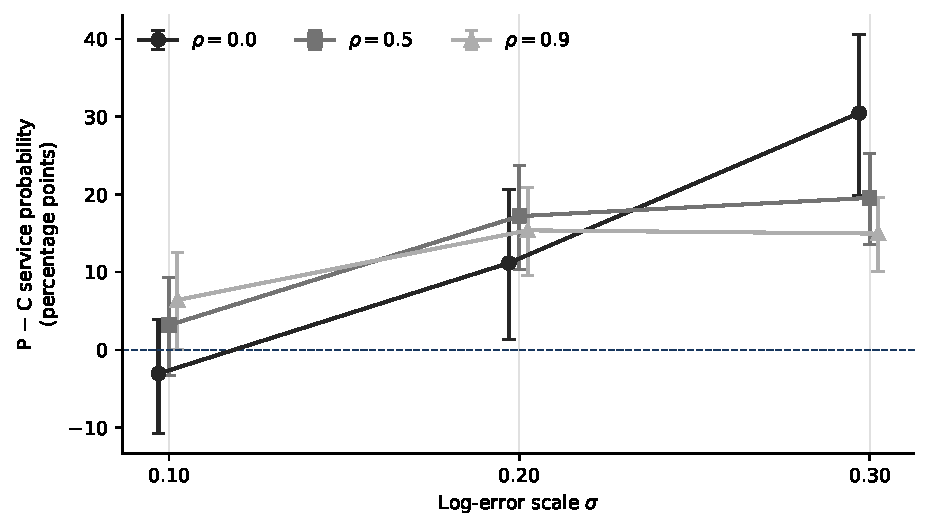
\includegraphics[width=0.8\textwidth]{../paper/Fig1.pdf}
\caption{Difference in validated reliability between the original procedure and
20\% padding on the 46 development instances, as the delay spread $\sigma$ and the
day-common share $\rho$ vary. Plans are fixed; error bars are 95\% bootstrap
intervals over instances.}
\label{fig:sweep}
\end{figure}

The cap matters (Table~\ref{tab:screen}). On \FailureCount{} development instances the original
procedure admitted no plan, and on \CertifiedFailures{} of them the shortest-path
bound proved that a customer had become unreachable at a large buffer. Capping
raised the instances with a passing plan from \OriginalSelected{} to
\CappedSelected{} and pooled service by \CappedGainInterval{} points, and at 100 and 200 customers the capped procedure
found a passing plan on every instance. The confirmatory studies repeated these
findings (Table~\ref{tab:primaries}). Seven of eight primary hypotheses were
confirmed: screening beat 20\% padding by \ConfHOneMean{} points on new instances,
capping added \ConfHTwoMean{} points, and with HGS the capped procedure beat padding
by \CtwoGOneMean{} points. The one hypothesis not confirmed (G2) was that falling
back to 20\% padding instead of the slack-aware plan would help the capped OR-Tools
procedure; it rarely needed a fallback. The best-screened fallback, tested in study
3B, raised pooled service by \PbFOne{} and \PbFTwo{} points for the two solvers.

\begin{table}[t]
\centering
\footnotesize
\setlength{\tabcolsep}{4pt}
\caption{Development study, all 53 instances. For each procedure: instances admitted by screening out of all instances of that size, with the number whose lower bound also reached 0.95 on the validation bank in parentheses, and pooled validated service probability (\%) with a 95\% bootstrap interval, fallback plans included.}
\label{tab:screen}
\begin{tabular}{@{}rllllll@{}}
\toprule
 & \multicolumn{2}{l}{Original procedure} & \multicolumn{2}{l}{Screened conservative} & \multicolumn{2}{l}{Capped procedure}\\
$n$ & Admitted & Pooled & Admitted & Pooled & Admitted & Pooled\\
\midrule
20 & 14/20 (14) & 81.6 [70.2, 91.9] & 15/20 (15) & 87.7 [79.0, 94.7] & 14/20 (14) & 81.6 [70.3, 92.0]\\
50 & 8/15 (8) & 72.7 [59.2, 86.4] & 4/15 (4) & 67.5 [58.2, 77.3] & 10/15 (10) & 80.1 [66.9, 90.8]\\
100 & 6/10 (5) & 81.3 [68.8, 93.3] & 4/10 (4) & 77.5 [67.2, 88.2] & 10/10 (9) & 97.5 [96.7, 98.2]\\
200 & 4/8 (3) & 80.6 [68.7, 92.3] & 2/8 (2) & 78.3 [71.0, 86.5] & 8/8 (7) & 97.6 [96.9, 98.2]\\
\bottomrule
\end{tabular}
\end{table}

\begin{table}[t]
\centering
\small
\caption{The eight primary hypotheses of the three confirmatory studies. Each was fixed and publicly timestamped before its instances were solved. Estimates are differences in validated service probability (percentage points) with 97.5\% paired bootstrap intervals over instances; a hypothesis is confirmed when its interval lies above zero.}
\label{tab:primaries}
\begin{tabular}{@{}cl>{\raggedright\arraybackslash}p{7.2cm}>{\raggedright\arraybackslash}p{2.9cm}l@{}}
\toprule
Study & & Contrast & Estimate [interval] & Decision\\
\midrule
1 & H1 & Original procedure minus 20\% padding (\ConfCommon{} instances) & \ConfHOneMean{} [\ConfHOneLo, \ConfHOneHi] & confirmed\\
1 & H2 & Capped minus original procedure (\ConfInstances{} instances) & \ConfHTwoMean{} [\ConfHTwoLo, \ConfHTwoHi] & confirmed\\
2 & G1 & Capped procedure with HGS minus 20\% padding with HGS (\CtwoCommon{} instances) & \CtwoGOneMean{} [\CtwoGOneLo, \CtwoGOneHi] & confirmed\\
2 & G2 & Conservative minus slack-aware fallback, capped OR-Tools procedure & \CtwoGTwoMean{} [\CtwoGTwoLo, \CtwoGTwoHi] & not confirmed\\
3A & R1 & Screened robust model minus capped OR-Tools procedure (\PaInstances{} instances) & \PaROne{} [\PaROneLo, \PaROneHi] & confirmed\\
3A & R2 & Screened robust model minus capped HGS procedure (45 instances) & \PaRTwo{} [\PaRTwoLo, \PaRTwoHi] & confirmed\\
3B & F1 & Best-screened minus default fallback, capped OR-Tools procedure & \PbFOne{} [\PbFOneLo, \PbFOneHi] & confirmed\\
3B & F2 & Best-screened minus default fallback, capped HGS procedure & \PbFTwo{} [\PbFTwoLo, \PbFTwoHi] & confirmed\\
\bottomrule
\end{tabular}
\end{table}


\subsection{Fixed padding at other levels}

A 20\% pad may simply be the wrong amount, so Table~\ref{tab:padding} and
Figure~\ref{fig:padding} repeat the comparison with padding from 0 to 50\%. Over all
instances no level came close to the capped procedure: the best, \PadBestLevel\%,
pooled \PadBestPooled\% against \PadCapPooled\%. More padding did not keep helping,
because heavy padding makes many instances impossible to plan; at 50\% the padded
planner found a plan on only \PadFiftyPlans{} of \PadInstances{} instances. These
failures are mostly real rather than failures of the search: of the \PfMissing{}
missing padded plans across all levels, \PfProven{} are provably infeasible, because at
the padded speed some customer cannot be reached within its window or within the
shift (at 50\%, \PfFiftyProven{} of \PfFiftyMissing); the other \PfUnresolved{} are
unresolved. Where it
did find one, the plan was reliable: on those instances 50\% padding served
\PadFiftyOnPlans\% against \PadFiftyCapOnPlans\% for screening, and used
\PadFiftyFleet{} more vehicles. A planner who fixes one padding level must choose
between unreliable plans at low levels and missing plans at high ones.

\begin{table}[t]
\centering
\small
\setlength{\tabcolsep}{4pt}
\caption{Padding every trip by a fixed percentage on the 53 development instances (exploratory). \emph{Plans}: instances on which the padded planner found a plan. \emph{All}: pooled service over all instances, an instance without a plan scoring zero. The next three columns use only the instances with a padded plan: the padded plans' service, the capped screening procedure's service on the same instances, and the difference (padding minus screening, percentage points, 95\% paired bootstrap interval). Distance (\%) and vehicles are also padding minus screening on those instances. Over all instances the capped procedure pooled 86.6\%.}
\label{tab:padding}
\begin{tabular}{@{}rrrrrlrr@{}}
\toprule
 & & \multicolumn{1}{c}{All} & \multicolumn{3}{c}{Instances with a padded plan} & & \\
\cmidrule(lr){3-3}\cmidrule(lr){4-6}
Padding & Plans & Pooled & Padded & Screened & Difference & Distance & Vehicles\\
\midrule
0\% & 53/53 & 21.9 & 21.9 & 86.6 & $-$64.7 [$-$70.2, $-$58.8] & $-$7.1 & $-$0.89\\
10\% & 51/53 & 43.7 & 45.4 & 88.4 & $-$42.9 [$-$48.0, $-$37.4] & $-$6.2 & $-$0.59\\
20\% & 46/53 & 56.8 & 65.4 & 89.4 & $-$23.9 [$-$29.2, $-$18.2] & $-$4.8 & $-$0.22\\
30\% & 43/53 & 66.7 & 82.2 & 90.3 & $-$8.1 [$-$13.1, $-$2.4] & $-$3.1 & 0.21\\
40\% & 34/53 & 58.8 & 91.6 & 88.5 & 3.1 [$-$2.8, 10.0] & $-$1.0 & 0.47\\
50\% & 26/53 & 47.1 & 96.1 & 87.9 & 8.2 [1.2, 16.1] & 0.9 & 0.77\\
\bottomrule
\end{tabular}
\end{table}


\begin{figure}[t]
\centering
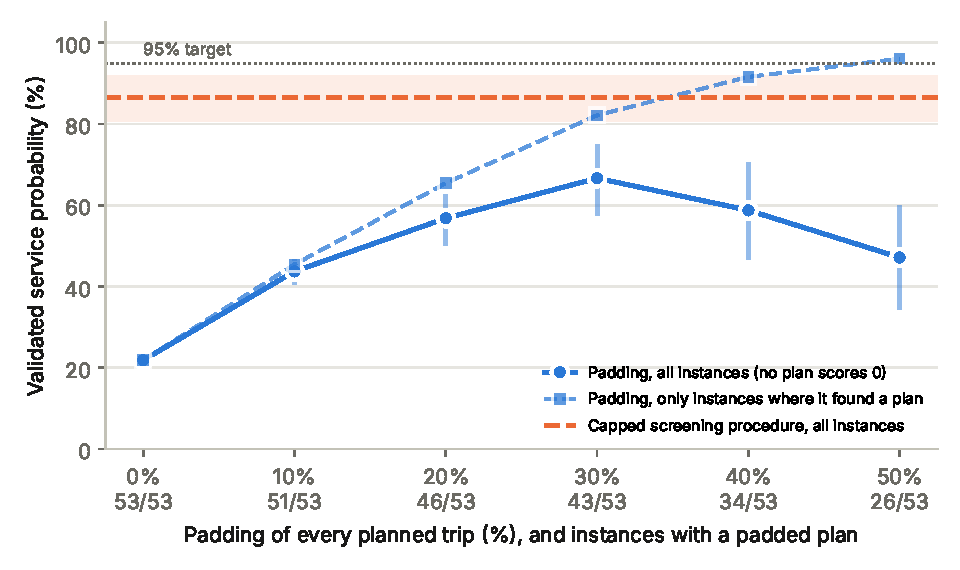
\includegraphics[width=0.8\textwidth]{FigPadding.pdf}
\caption{Validated reliability against fixed padding on the 53 development
instances. Solid line: all instances, a missing plan scoring zero; dashed line:
only instances where a padded plan exists (counts under the axis). Orange line and
band: the capped procedure over all instances, with its 95\% bootstrap interval.}
\label{fig:padding}
\end{figure}

\subsection{Certification}\label{sec:cert-results}

Table~\ref{tab:certify} applies the certificate to every configuration in every
study. The capped procedure was certified on \CertDevCap{} of 53 development
instances and on \CertConeCap{} and \CertCtwoCap{} of 53 in the two confirmatory
studies; its HGS version on \CertDevHCap{} and \CertCtwoHCap. Twenty percent padding
was never certified on a synthetic instance (0 of \CertPadSynN{} plans): its plans
are often good, but rarely good enough to show 95\% with confidence. On the Amazon
routes the picture depends on the delay model, which we return to below. Across
the table, \CertTotal{} plans were certified. On 5000 fresh days, none of them failed
its certificate, and only \CertBelow{} had a fresh success rate below 0.95, all
within sampling error of it. The theorem would have allowed about 5\% failures; the
observed rate is lower because most certified plans are well above the target.
Because the fresh days come from the same delay model, this test checks the
implementation and the statistics, not the model; the test that matters in
practice is the one in Section~\ref{sec:wrong}.

\begin{table}[t]
\centering
\small
\setlength{\tabcolsep}{4pt}
\caption{Certified plans: plans whose exact one-sided 95\% lower bound on the success probability, from the 5000 validation days, is at least 0.95, out of the plans the configuration produced. Dev., Conf.~1 and Conf.~2: development and first two confirmatory studies (53 instances each); Amazon: 40 routes under the assumed delay model and under the two models fitted to New York traffic. On a further 5000 fresh days, none of the 666 certified plans in the table failed its certificate (exact one-sided 95\% upper bound below 0.95).}
\label{tab:certify}
\begin{tabular}{@{}lcccccc@{}}
\toprule
Configuration & Dev. & Conf.\ 1 & Conf.\ 2 & Amazon & NYC d. & NYC all\\
\midrule
Nominal plan (OR-Tools) & 0/53 & 0/53 & 0/53 & 0/34 & 3/34 & 0/34\\
20\% padding (OR-Tools) & 0/46 & 0/50 & 0/45 & 0/28 & 28/28 & 4/28\\
Original procedure & 30/53 & 31/53 & 28/53 & 22/34 & 33/34 & 29/34\\
Capped procedure & 40/53 & 45/53 & 45/53 & 22/34 & 33/34 & 29/34\\
Screened conservative & 25/53 & 28/53 & 26/53 & 24/34 & 30/34 & 23/34\\
Nominal plan (HGS) & 0/53 & -- & 0/53 & -- & -- & --\\
20\% padding (HGS) & 0/48 & -- & 0/49 & -- & -- & --\\
Capped procedure (HGS) & 46/53 & -- & 42/53 & -- & -- & --\\
\bottomrule
\end{tabular}
\end{table}


\subsection{The cost of reliability}\label{sec:frontier}

Table~\ref{tab:frontier} and Figure~\ref{fig:frontier} ask which reliability each
family can reach on an instance, and at what cost. At 90\% the buffer family
contains a qualifying plan on \FrBufNinety{} of \FrN{} instances and the padding
family on \FrPadNinety; at 95\% on \FrBufNinetyFive{} and \FrPadNinetyFive; with the
exact lower bound at 95\% on \FrBufCert{} and \FrPadCert; and at 99\% on \FrBufNinetyNine{}
and \FrPadNinetyNine. Where both families reach 95\%, the cheapest buffered plan
used \FrFleetNinetyFiveAbs{} fewer vehicles [\FrFleetNinetyFiveAbsLo,
\FrFleetNinetyFiveAbsHi] but \FrDistNinetyFive\% more distance [\FrDistNinetyFiveLo,
\FrDistNinetyFiveHi] than the cheapest padded plan. At reliability levels of 80\% or
less, buffers were cheaper in both. Padding buys reliability by slowing every trip,
which eventually costs vehicles; a buffer spends time only where the internal
deadline binds.

\begin{table}[t]
\centering
\small
\setlength{\tabcolsep}{4pt}
\caption{The cost of reliability on the 53 development instances. For each level, the number of instances on which the buffer family (13 capped candidates) and the padding family (0 to 50\%) contain a plan whose validated success probability reaches it, and, where both do, the paired difference in cost between the cheapest such plans (buffers minus padding): distance in percent of the plain distance plan, and vehicles. 95\% bootstrap intervals over instances. \emph{Exact bound}: the Clopper--Pearson lower bound, rather than the estimate, must reach 95\%; because the plan is chosen on the same days, this row is descriptive and is not a certificate in the sense of Theorem~\ref{thm:cert}.}
\label{tab:frontier}
\begin{tabular}{@{}lccclll@{}}
\toprule
 & \multicolumn{2}{c}{Instances reached} & & \multicolumn{2}{c}{Buffers minus padding} \\
\cmidrule(lr){2-3}\cmidrule(lr){5-6}
Reliability & Buffers & Padding & Both & Distance (\%) & Vehicles\\
\midrule
50\% & 52 & 47 & 47 & $-$1.0 [$-$1.7, $-$0.3] & $-$0.45 [$-$0.72, $-$0.19]\\
70\% & 51 & 43 & 43 & $-$1.4 [$-$2.3, $-$0.5] & $-$0.65 [$-$1.05, $-$0.30]\\
80\% & 51 & 42 & 42 & $-$1.2 [$-$2.1, $-$0.4] & $-$0.79 [$-$1.10, $-$0.50]\\
90\% & 50 & 33 & 32 & 0.1 [$-$1.2, 1.5] & $-$0.75 [$-$1.22, $-$0.34]\\
95\% & 46 & 23 & 22 & 1.5 [0.2, 2.9] & $-$0.64 [$-$1.09, $-$0.23]\\
95\%, exact bound & 45 & 20 & 19 & 1.8 [0.3, 3.4] & $-$0.58 [$-$1.00, $-$0.21]\\
99\% & 29 & 0 & 0 & -- & --\\
\bottomrule
\end{tabular}
\end{table}


\begin{figure}[t]
\centering
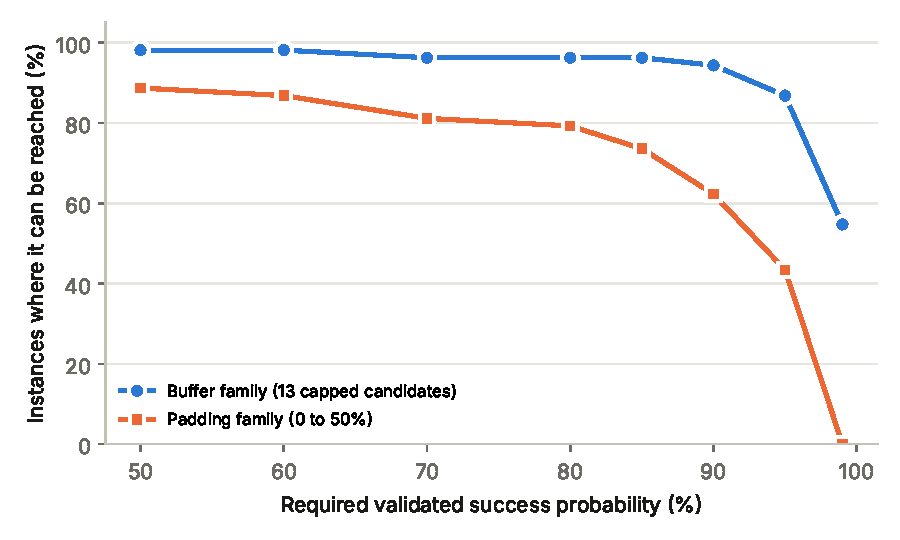
\includegraphics[width=0.75\textwidth]{FigFrontier.pdf}
\caption{Share of the \FrN{} development instances on which some plan of each family
reaches a required validated reliability.}
\label{fig:frontier}
\end{figure}

\subsection{Benchmark instances}

On R1\_2\_1 and R1\_2\_2, where all or most windows are only 10 time units wide,
neither the anchor solves nor HGS at padded speed found a plan. Screening admitted a
plan on \GhAdmitted{} of the other \GhAttempted{} instances (Table~\ref{tab:gh}), and
on those instances the capped HGS procedure exceeded 20\% padding by \GhDiff{}
[\GhDiffLo, \GhDiffHi] points; over all 20 it pooled \GhCapped\% against \GhCons\%.

\begin{table}[t]
\centering
\footnotesize
\setlength{\tabcolsep}{4pt}
\caption{Gehring--Homberger instances with 200 customers (exploratory, HGS pipeline): instances, instances where the four single-criterion solves that set the objective's scaling ranges (the anchors) all found a plan, instances admitted by screening, and pooled validated service-event probability (\%) of the HGS nominal plan, HGS conservative speed and the HGS capped procedure with conservative fallback. A missing plan scores zero.}
\label{tab:gh}
\begin{tabular}{@{}lrrrrrr@{}}
\toprule
Class & Inst. & Anchors & Admitted & Nominal & Conservative & Capped\\
\midrule
R1 & 10 & 8 & 7 & 42.1 & 68.0 & 77.0\\
RC1 & 10 & 10 & 10 & 27.6 & 79.3 & 97.4\\
\bottomrule
\end{tabular}
\end{table}


\subsection{Real delivery routes}\label{sec:amazon-results}

Table~\ref{tab:nyc} gives the delay model fitted to New York traffic. It differs
from the assumed one in one important way: the rush hours were not slower than the
middle of the day. Trips between 07:00 and 09:00 were \NycAmFaster\% faster and
trips between 17:00 and 19:00 \NycPmFaster\% faster than between 09:00 and 17:00.
The assumed spread of 0.20 lies between the two fitted values.

\begin{table}[t]
\centering
\small
\caption{The delay model fitted to 6.2 million weekday New York yellow-taxi trips (January--March 2024). Time-of-day multipliers of travel time relative to 09:00--17:00, from zone pairs with at least 20 trips in both periods; the spread $\sigma$ and the day-common share $\rho$ of the random factor are estimated in two ways (see text).}
\label{tab:nyc}
\begin{tabular}{@{}lccr@{}}
\toprule
Period & Assumed & Fitted & Zone pairs\\
\midrule
00:00--07:00 & 0.9 & 0.62 & 2{,}669\\
07:00--09:00 & 1.2 & 0.84 & 2{,}424\\
09:00--17:00 & 1.0 & 1.00 & 4{,}603\\
17:00--19:00 & 1.3 & 0.94 & 3{,}237\\
19:00--24:00 & 0.9 & 0.76 & 3{,}865\\
\midrule
$\sigma$ & 0.20 & 0.11 (day to day), 0.27 (all) & \\
$\rho$ & 0.50 & 0.40 (day to day), 0.06 (all) & \\
\bottomrule
\end{tabular}
\end{table}


On the Amazon routes (Table~\ref{tab:amazon}), the capped procedure was more
reliable than 20\% padding under every delay model: by \AmzCapDiff{}
[\AmzCapDiffLo, \AmzCapDiffHi] points under the assumed model, \AmzDCapDiff{}
[\AmzDCapDiffLo, \AmzDCapDiffHi] with the fitted day-to-day variation and
\AmzTCapDiff{} [\AmzTCapDiffLo, \AmzTCapDiffHi] with all fitted variation. Much of
this gap comes from planning: padding produced no plan on \AmzConsNoPlan{} routes,
against \AmzNoPlan{} for the other configurations. On the \AmzBoth{} routes where
both had a plan, the two were level under the assumed model (\AmzBothDiff{}
[\AmzBothDiffLo, \AmzBothDiffHi] points), screening was ahead with all fitted
variation (\AmzTBothDiff{} [\AmzTBothDiffLo, \AmzTBothDiffHi]), and with the
milder day-to-day variation padding was slightly more reliable (\AmzDBothDiff{}
[\AmzDBothDiffLo, \AmzDBothDiffHi]); under that model \CertAmzDPad{} of the
\CertAmzDPadN{} padded plans were certified (Table~\ref{tab:certify}). When no candidate passed, the capped procedure's
slack-aware fallback was weaker than padding (\AmzCapOnFallback\% against
\AmzConsOnFallback\% under the assumed model), which screened conservative avoids
because its fallback is the padded plan.

On \AmzNoPlan{} routes with \AmzNoPlanCustMin{} to \AmzNoPlanCustMax{} customers no
configuration found a plan, although the driver's own order is feasible by
construction, so these are limits of the solver's search. A longer search changes
part of the comparison. Given \SrchSeconds{} seconds per attempt instead of 5,
OR-Tools still found no nominal plan on these \SrchNomMissing{} routes, but it found a
20\% padded plan on \SrchConsFound{} of the \SrchConsMissing{} routes where padding
had none. Re-scoring padding with these plans, while keeping the screened procedures
at their 5-second budget, the capped procedure's lead became \SrchDiff{}
[\SrchDiffLo, \SrchDiffHi] points under the assumed model, \SrchDDiff{}
[\SrchDDiffLo, \SrchDDiffHi] with the fitted day-to-day variation and \SrchTDiff{}
[\SrchTDiffLo, \SrchTDiffHi] with all fitted variation. With OR-Tools, therefore,
the comparison on real routes is clouded by the solver's search.

\begin{table}[t]
\centering
\small
\setlength{\tabcolsep}{4pt}
\caption{Real delivery routes: 40 Amazon routes from five US cities (exploratory), under the assumed delay model and under the two delay models fitted to New York taxi trips (Table~\ref{tab:nyc}). \emph{Plans}: routes on which the configuration produced a plan (the same under every delay model). Pooled validated service probability (\%) with a 95\% bootstrap interval over routes; a route without a plan scores zero. \emph{Admitted}: routes on which a candidate passed the screen.}
\label{tab:amazon}
\begin{tabular}{@{}lclll@{}}
\toprule
 & & \multicolumn{3}{c}{Pooled service under the delay model} \\
Configuration & Plans & Assumed & NYC, day to day & NYC, all variation\\
\midrule
Nominal plan (no protection) & 34/40 & 41.4 [35.1, 47.1] & 64.9 [55.4, 73.5] & 46.9 [39.6, 53.8]\\
20\% padding & 28/40 & 59.0 [46.6, 70.8] & 69.5 [54.7, 82.2] & 59.5 [46.8, 71.8]\\
Capped screening procedure & 34/40 & 72.6 [61.2, 82.9] & 83.4 [71.3, 93.3] & 80.1 [68.5, 90.2]\\
Screened conservative & 34/40 & 75.3 [63.6, 85.7] & 83.2 [71.3, 93.3] & 77.3 [65.9, 87.5]\\
\midrule
Admitted, capped procedure & & 24 & 34 & 30\\
Admitted, screened conservative & & 25 & 28 & 26\\
\bottomrule
\end{tabular}
\end{table}


The HGS solver removes that problem, so it gives the fairer comparison
(Table~\ref{tab:amazonhgs}). It was run on all \AmzHRoutes{} sampled routes, the 40
above and the 20 spares, and found a 20\% padded plan on every route. On
\AmzHNotRun{} routes the short OR-Tools solves that set the objective's scaling ranges
failed, so the screen could not run and the procedure returned its fallback, the
padded plan. On the \AmzHBoth{} routes where the screen ran, the capped HGS procedure
was \AmzHBothDiff{} [\AmzHBothDiffLo, \AmzHBothDiffHi] points more reliable than
padding under the assumed model and \AmzHTBothDiff{} [\AmzHTBothDiffLo,
\AmzHTBothDiffHi] points more reliable with all fitted variation, with practically the
same number of vehicles. With the milder fitted day-to-day variation padding was
slightly ahead (screening minus padding \AmzHDBothDiff{} [\AmzHDBothDiffLo,
\AmzHDBothDiffHi] points): delays were small enough that \AmzHDCertPad{} of
\AmzHPadPlans{} padded plans were certified, which leaves little for screening to add. Over all
routes, counting the fallback, the differences were \AmzHFbDiff, \AmzHDFbDiff{} and
\AmzHTFbDiff{} points. The certificate behaved as on the synthetic instances: none of
the certified plans failed on fresh days. The real-route evidence is therefore
consistent with the synthetic studies: screening helps when delays are large
enough to matter, and when they are not, padding is already reliable and the
certificate says so.

\begin{table}[t]
\centering
\small
\setlength{\tabcolsep}{3.5pt}
\caption{The 60 Amazon routes with the HGS solver (exploratory). \emph{Padding} and \emph{Capped}: pooled validated reliability (\%) of 20\% padding and of the capped HGS procedure, which falls back to padding on the 12 routes where its scaling solves failed and the screen could not run. \emph{All}: capped minus padding over all routes; \emph{Both}: the same on the routes where the screen ran, with the difference in vehicles. \emph{Certified}: plans certified, padding and capped. 95\% bootstrap intervals.}
\label{tab:amazonhgs}
\begin{tabular}{@{}lccllccc@{}}
\toprule
 & & & \multicolumn{2}{c}{Capped minus padding} & & \multicolumn{2}{c}{Certified}\\
\cmidrule(lr){4-5}\cmidrule(lr){7-8}
Delay model & Padding & Capped & All & Both & Vehicles & Pad. & Cap.\\
\midrule
Assumed & 85.0 & 91.4 & 6.4 [4.3, 8.6] & 8.0 [5.6, 10.5] & 0.04 & 0 & 26\\
NYC, day to day & 99.4 & 98.4 & $-$1.0 [$-$1.4, $-$0.6] & $-$1.2 [$-$1.7, $-$0.8] & $-$0.21 & 60 & 45\\
NYC, all variation & 86.8 & 94.9 & 8.1 [5.5, 10.9] & 10.1 [7.1, 13.4] & 0.02 & 14 & 42\\
\bottomrule
\end{tabular}
\end{table}


\subsection{When the delay model is wrong}\label{sec:wrong}

A firm screens with the delay model it has, and real delays differ. The top of
Table~\ref{tab:wrong} takes the Amazon plans chosen under the assumed model and
judges them, on fresh days, under the models fitted to New York traffic. They
stayed ahead of padding at the same 5-second budget, by \WrDCapPad{} [\WrDCapPadLo,
\WrDCapPadHi] and \WrTCapPad{} [\WrTCapPadLo, \WrTCapPadHi] points for the capped
procedure, a margin that a longer search for padding would reduce
(Section~\ref{sec:amazon-results}). Screening
with the right model instead added only \WrDGain{} [\WrDGainLo, \WrDGainHi] and
\WrTGain{} [\WrTGainLo, \WrTGainHi] points. Every certificate granted under the
assumed model still held under both fitted models (\WrDCapKept{} of \WrDCapCert{}
for the capped procedure and \WrDScKept{} of \WrDScCert{} for screened
conservative).

This is the favourable direction, because the assumed model is harsher than New
York traffic in the morning. The bottom of the table shows the other direction, on
the synthetic instances, with delay models chosen before the analysis. Certificates
survived heavy-tailed delays (\WrTailKept{} of \WrTailCert) and mostly survived more
noise in the peaks (\WrNoiseKept{} of \WrNoiseCert). They often failed when 3\% of
trips suffered an incident that doubled their time (\WrIncKept{} of \WrIncCert{}
kept) and when the morning peak was stronger than planned (\WrPeakKept{} of
\WrPeakCert{} kept), although the certified plans still averaged \WrIncServ\% and
\WrPeakServ\% reliability under those models, against \WrIncPad\% and \WrPeakPad\% for 20\%
padding over all \WrIncPadN{} synthetic instances. The certificate is therefore exactly as good as the delay model's
pessimism: it carries over to milder or differently shaped delays, but not to delays
that are systematically worse than modelled, as
Proposition~\ref{prop:transfer} leads one to expect.

\begin{table}[t]
\centering
\small
\setlength{\tabcolsep}{4pt}
\caption{When the delay model is wrong. Top: the 40 Amazon routes, judged on 5000 fresh days under each delay model fitted to New York traffic. \emph{Wrong}: plans chosen when the screen used the assumed model; \emph{Right}: plans chosen when it used the fitted model. Pooled service (\%), and certificates (granted under the model used for screening) that still hold. Bottom: plans certified under the assumed model on the synthetic instances of the development and confirmatory studies, judged under delay models that differ from it; certificates that still hold and the mean service (\%) of the certified plans.}
\label{tab:wrong}
\begin{tabular}{@{}lcccccc@{}}
\toprule
 & \multicolumn{3}{c}{NYC, day-to-day variation} & \multicolumn{3}{c}{NYC, all variation}\\
\cmidrule(lr){2-4}\cmidrule(lr){5-7}
 & Wrong & Kept & Right & Wrong & Kept & Right\\
\midrule
20\% padding & 69.5 & -- & 69.5 & 59.5 & -- & 59.5\\
Capped procedure & 81.8 & 22/22 & 83.4 & 76.4 & 22/22 & 80.1\\
Screened conservative & 83.4 & 24/24 & 83.1 & 77.3 & 24/24 & 77.4\\
\midrule
 & \multicolumn{2}{c}{Capped (OR-Tools)} & \multicolumn{2}{c}{Capped (HGS)} & & \\
\cmidrule(lr){2-3}\cmidrule(lr){4-5}
True delay model & Kept & Service & Kept & Service & & \\
\midrule
Assumed model (new days) & 130/130 & 97.6 & 88/88 & 97.5 & & \\
Heavy-tailed delays & 130/130 & 97.5 & 88/88 & 97.3 & & \\
More noise in the peaks & 102/130 & 95.9 & 66/88 & 95.7 & & \\
Random incidents & 44/130 & 93.3 & 17/88 & 92.6 & & \\
Stronger morning peak & 52/130 & 93.7 & 22/88 & 93.2 & & \\
\bottomrule
\end{tabular}
\end{table}


Proposition~\ref{prop:multi} offers a remedy, tested in Table~\ref{tab:stress} with
the same five delay models. Here the ordinary certificate is granted on the
5000-day banks of the misspecification analysis, which certifies
\StOSingle{} OR-Tools plans; on fresh days \StOSingleIncFail{} of them failed under
random incidents and \StOSinglePeakFail{} under the stronger peak. Requiring the
plans the ordinary screen selected to be certified under all five models keeps only
\StOSingleAll{} of \StOInst{}. The \emph{stress screen}, which admits a candidate only
if it passes under all five models and then certifies it under all five, certified
\StOStress{} OR-Tools plans and \StHStress{} HGS plans, and none of them failed its
certificate on fresh days under any of the five models (\StStressFails{} failures in
total). Under random incidents and the stronger peak these plans averaged
\StOIncServ\% and \StOPeakServ\% reliability. Robustness has a price: on the
\StOBoth{} instances where both screens selected a plan, the stress-screened OR-Tools
plan used \StOFleet{} more vehicles and \StODist\% more distance (HGS: \StHFleet{}
vehicles and \StHDist\%), and the stress screen certified a plan on \StOStress{} of
\StOInst{} instances instead of \StOSingle{} (HGS: \StHStress{} of \StHInst{} instead of
\StHSingle).

\begin{table}[t]
\centering
\small
\setlength{\tabcolsep}{4pt}
\caption{Certifying against several delay models, on the synthetic instances of the development and confirmatory studies. \emph{Certified}: plans certified, out of all instances. The other columns count certified plans that failed their certificate on 5000 fresh days under each true delay model: random incidents, a stronger morning peak, more noise in the peaks, heavy-tailed delays, and the assumed model. The stress screen admits a candidate only if it passes under all five models.}
\label{tab:stress}
\begin{tabular}{@{}>{\raggedright\arraybackslash}p{6.6cm}cccccc@{}}
\toprule
 & & \multicolumn{5}{c}{Failed certificates under the true model}\\
\cmidrule(lr){3-7}
Configuration & Certified & Incid. & Peak & Noise & Tails & Assumed\\
\midrule
\multicolumn{7}{@{}l}{\emph{Capped (OR-Tools)}}\\
\quad Ordinary screen, certified under the assumed model & 131/159 & 90 & 82 & 27 & 0 & 0\\
\quad Ordinary screen, certified under all five models & 15/159 & 0 & 0 & 0 & 0 & 0\\
\quad Stress screen, certified under all five models & 76/159 & 0 & 0 & 0 & 0 & 0\\
\multicolumn{7}{@{}l}{\emph{Capped (HGS)}}\\
\quad Ordinary screen, certified under the assumed model & 90/106 & 69 & 69 & 24 & 0 & 0\\
\quad Ordinary screen, certified under all five models & 12/106 & 0 & 0 & 0 & 0 & 0\\
\quad Stress screen, certified under all five models & 42/106 & 0 & 0 & 0 & 0 & 0\\
\bottomrule
\end{tabular}
\end{table}


\subsection{Comparison with robust optimization}

A budgeted robust model plans against worst-case travel times on a limited number of
trips. Without a reachability correction it failed on \RobNoPlanBoxSix{} of
\RobInstances{} development instances at its most protective setting, for the same
reason as the uncapped procedure. With an analogous correction and the same screen,
the robust plans were more reliable than both screened procedures in study 3 part A
(by \PaROne{} and \PaRTwo{} points; Table~\ref{tab:primaries}), but used \PaRThree{}
more vehicles per instance than the HGS procedure, and when limited to no more
vehicles than the comparison plan their advantage was no longer detectable. The
layer is therefore not the most reliable planner tested; its value is that it works
with the solver a firm already has, and that it says how reliable the plan is.

\section{Implications for planning systems}\label{sec:implications}

For a firm, the layer sits between the routing solver and dispatch. It needs no
change to the solver, only the ability to tighten internal deadlines and to
simulate plans, and screening a candidate took \TimeScreenTwenty{} to
\TimeScreenTwoHundred{}~ms against several seconds to generate it. Four practical
rules follow from the results. First, report the certificate, not only the plan: a
certified plan comes with a guarantee that padding cannot give, and an uncertified
one is a warning that the day is at risk. Second, use the capped deadlines;
without them large buffers can make the problem infeasible for reasons that have
nothing to do with the fleet. Third, choose the fallback deliberately. The
best-screened candidate was the confirmed improvement in the synthetic studies, and
on the Amazon routes falling back to the padded plan was safer than the unbuffered
one; in either case the plan returned is not certified and should be flagged.
Fourth, certify against delay models that are at least as harsh as reality. A
certificate carries over to milder delays (Proposition~\ref{prop:transfer}) but not
to harsher ones, so a firm should screen and certify against a small set of
models, for example its fitted model together with incidents and a stronger peak
(Proposition~\ref{prop:multi}), and accept the extra vehicles this costs.

\section{Limitations}\label{sec:limitations}

The main studies use synthetic instances and an assumed delay model; the benchmark
and Amazon experiments show that the findings are not specific to the generator or
to the assumed model, but the Amazon windows are assumed, and the fitted delays
come from New York taxis rather than from the cities where the routes were driven.
The certificate is relative to the simulated model, as Section~\ref{sec:wrong}
shows. All analyses beyond the eight primary hypotheses are exploratory. The
advantage depends on the planner's objective: with equal weights on the four
criteria it fell to \WtEqualPCMean{} points, with an interval that included zero.
Vehicles always leave at their planned times, and breakdowns and same-day
re-planning are not modelled. Finally, OR-Tools with a 5-second limit missed
feasible plans on some Amazon routes, and the scaling solves that the weighted
objective needs failed on \AmzHNotRun{} of \AmzHRoutes{} routes, so the screen could not
run there; with HGS the reliability gain on real routes was clear under two of the
three delay models, and under the mildest one padding was already reliable.

\section{Conclusion}\label{sec:conclusion}

A firm can add a reliability guarantee to the routing solver it already uses. Asking
the solver for a few plans with capped internal buffers, screening them by
simulation and certifying the chosen plan on independent days gave more reliable
service than fixed padding at any level on the synthetic instances, reached high
reliability on twice as many instances with fewer vehicles, and produced certificates that held on fresh days
without exception in our studies. The guarantee is about the delay model, but it
carries over to any real delays no worse than modelled, and certifying against a
small set of pessimistic models removed every failure we observed, at a cost of
less than one vehicle per instance. The models should be estimated from the firm's
own trips. Testing the layer on a fleet's own travel-time records, with its real
delivery windows, is the natural next step.

\ifanonymous\else
\section*{Acknowledgements}
The author thanks the researchers who answered methodological questions by e-mail
during the project.
\fi

\section*{Use of generative AI}
Anthropic's Claude and OpenAI's ChatGPT were used to write and debug the simulation
and analysis code, to review that code, to run and check the statistical analyses,
to search the literature, and to draft and revise the text of this manuscript,
including its wording. The research question, the study design and the
confirmatory protocols were the author's. Every experiment was run from the
archived code, every reported number is regenerated from the archived records, and
the author takes full responsibility for the content.

\section*{Disclosure statement}
The author reports there are no competing interests to declare.

\section*{Funding}
This research received no external funding.

\section*{Data availability statement}
\ifanonymous
All code, instances, records and analysis scripts are openly available in a public
archive \citep{ali2026archive}; the identifier is withheld for review.
\else
All code, instances, records and analysis scripts are openly available
\citep{ali2026archive}. The Amazon route sample is redistributed under its
CC~BY-NC~4.0 licence; the New York taxi records are public and are not copied.
\fi

\bibliographystyle{plainnat}
\bibliography{\refsfile}

\end{document}
